\documentclass[tikz,margin=2mm]{standalone}
\pagestyle{empty}

\usepackage{amsmath}
\usepackage{bm}
\usetikzlibrary{positioning,calc,arrows,arrows.meta}
\tikzset{font=\small}

\begin{document}

	% Example a True DAG
	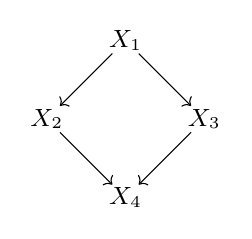
\begin{tikzpicture}
	\begin{scope}
		\tikzstyle{every node}=[align=center, inner sep=1pt]
		\node (x1) at (0, 0) {$X_1$};
		\node (x2) at (-1, -1) {$X_2$};
		\node (x3) at (1, -1) {$X_3$};
		\node (x4) at (0, -2) {$X_4$};

		\draw[->] (x1) -- (x2);
		\draw[->] (x1) -- (x3);
		\draw[->] (x2) -- (x4);
		\draw[->] (x3) -- (x4);

	\end{scope}
	\end{tikzpicture}

	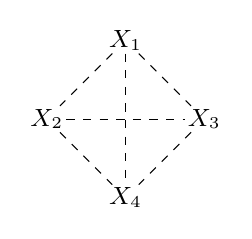
\begin{tikzpicture}
	\begin{scope}
		\tikzstyle{every node}=[align=center, inner sep=1pt]
		\node (x1) at (0, 0) {$X_1$};
		\node (x2) at (-1, -1) {$X_2$};
		\node (x3) at (1, -1) {$X_3$};
		\node (x4) at (0, -2) {$X_4$};

		\draw[dashed] (x1) -- (x2);
		\draw[dashed] (x1) -- (x3);
		\draw[dashed] (x2) -- (x4);
		\draw[dashed] (x3) -- (x4);
		\draw[dashed] (x1) -- (x4);
		\draw[dashed] (x2) -- (x3);

	\end{scope}
	\end{tikzpicture}


	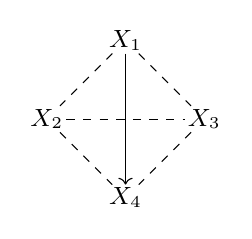
\begin{tikzpicture}
	\begin{scope}
		\tikzstyle{every node}=[align=center, inner sep=1pt]
		\node (x1) at (0, 0) {$X_1$};
		\node (x2) at (-1, -1) {$X_2$};
		\node (x3) at (1, -1) {$X_3$};
		\node (x4) at (0, -2) {$X_4$};

		\draw[dashed] (x1) -- (x2);
		\draw[dashed] (x1) -- (x3);
		\draw[dashed] (x2) -- (x4);
		\draw[dashed] (x3) -- (x4);
		\draw[->] (x1) -- (x4);
		\draw[dashed] (x2) -- (x3);

	\end{scope}
	\end{tikzpicture}

	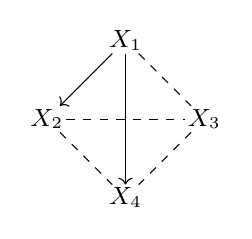
\begin{tikzpicture}
	\begin{scope}
		\tikzstyle{every node}=[align=center, inner sep=1pt]
		\node (x1) at (0, 0) {$X_1$};
		\node (x2) at (-1, -1) {$X_2$};
		\node (x3) at (1, -1) {$X_3$};
		\node (x4) at (0, -2) {$X_4$};

		\draw[->] (x1) -- (x2);
		\draw[dashed] (x1) -- (x3);
		\draw[dashed] (x2) -- (x4);
		\draw[dashed] (x3) -- (x4);
		\draw[->] (x1) -- (x4);
		\draw[dashed] (x2) -- (x3);

	\end{scope}
	\end{tikzpicture}

	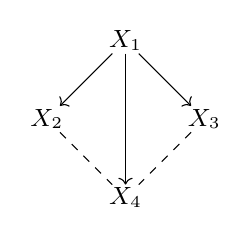
\begin{tikzpicture}
	\begin{scope}
		\tikzstyle{every node}=[align=center, inner sep=1pt]
		\node (x1) at (0, 0) {$X_1$};
		\node (x2) at (-1, -1) {$X_2$};
		\node (x3) at (1, -1) {$X_3$};
		\node (x4) at (0, -2) {$X_4$};

		\draw[->] (x1) -- (x2);
		\draw[->] (x1) -- (x3);
		\draw[dashed] (x2) -- (x4);
		\draw[dashed] (x3) -- (x4);
		\draw[->] (x1) -- (x4);

	\end{scope}
	\end{tikzpicture}

	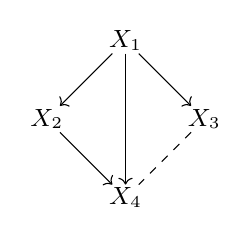
\begin{tikzpicture}
	\begin{scope}
		\tikzstyle{every node}=[align=center, inner sep=1pt]
		\node (x1) at (0, 0) {$X_1$};
		\node (x2) at (-1, -1) {$X_2$};
		\node (x3) at (1, -1) {$X_3$};
		\node (x4) at (0, -2) {$X_4$};

		\draw[->] (x1) -- (x2);
		\draw[->] (x1) -- (x3);
		\draw[->] (x2) -- (x4);
		\draw[dashed] (x3) -- (x4);
		\draw[->] (x1) -- (x4);

	\end{scope}
	\end{tikzpicture}

	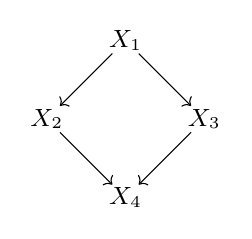
\begin{tikzpicture}
	\begin{scope}
		\tikzstyle{every node}=[align=center, inner sep=1pt]
		\node (x1) at (0, 0) {$X_1$};
		\node (x2) at (-1, -1) {$X_2$};
		\node (x3) at (1, -1) {$X_3$};
		\node (x4) at (0, -2) {$X_4$};

		\draw[->] (x1) -- (x2);
		\draw[->] (x1) -- (x3);
		\draw[->] (x2) -- (x4);
		\draw[->] (x3) -- (x4);
	\end{scope}
	\end{tikzpicture}

% 	% Example a True DAG
% 	\begin{tikzpicture}
% 	\begin{scope}
% 		\tikzstyle{every node}=[align=center, inner sep=1pt]
% 		\node (x1) at (0, 0) {$X_1$};
% 		\node (x2) at (0, -2) {$X_2$};
% 		\node (x3) at (1, -1) {$X_3$};
% 		\node (x4) at (2, 0) {$X_4$};
% 		\node (x5) at (2, -2) {$X_5$};
% 
% 		\draw[->, >=stealth](x1) -- (x3);
% 		\draw[->, >=stealth](x2) -- (x3);
% 		\draw[->, >=stealth](x3) -- (x4);
% 		\draw[->, >=stealth](x3) -- (x5);
% 	\end{scope}
% 	\end{tikzpicture}
% 
%	% Example  b
% 	\begin{tikzpicture}
% 	\begin{scope}
% 		\tikzstyle{every node}=[align=center, inner sep=1pt]
% 		\node (x1) at (0, 0) {$X_1$};
% 		\node (x2) at (0, -2) {$X_2$};
% 		\node (x3) at (1, -1) {$X_3$};
% 		\node (x4) at (2, 0) {$X_4$};
% 		\node (x5) at (2, -2) {$X_5$};
% 
% 		\draw[dashed, line width=0.5mm   ](x1) --                (x3);
% 		\draw[dashed, line width=0.25mm  ](x1) --                (x4);
% 		\draw[dashed, line width=0.25mm  ](x1) to[bend right=30] (x5);
% 		\draw[dashed, line width=0.5mm   ](x2) --                (x3);
% 		\draw[dashed, line width=0.25mm  ](x2) to[bend left=30]  (x4);
% 		\draw[dashed, line width=0.25mm  ](x2) --                (x5);	
% 		\draw[dashed, line width=0.5mm   ](x3) --                (x4);
% 		\draw[dashed, line width=0.5mm   ](x3) --                (x5);
% 		\draw[dashed, line width=0.25mm  ](x4) --                (x5);
% 	\end{scope}
% 	\end{tikzpicture}

		
% 	% Example  c
% 	\begin{tikzpicture}
% 	\begin{scope}
% 		\tikzstyle{every node}=[align=center, inner sep=1pt]
% 		\node (x1) at (0, 0) {$X_1$};
% 		\node (x2) at (0, -2) {$X_2$};
% 		\node (x3) at (1, -1) {$X_3$};
% 		\node (x4) at (2, 0) {$X_4$};
% 		\node (x5) at (2, -2) {$X_5$};
% 
% 		\draw[->, >=stealth              ](x1) --                (x3);
% 		\draw[dashed, line width=0.25mm  ](x1) --                (x4);
% 		\draw[dashed, line width=0.25mm  ](x1) to[bend right=30] (x5);
% 		\draw[dashed, line width=0.5mm   ](x2) --                (x3);
% 		\draw[dashed, line width=0.25mm  ](x2) to[bend left=30]  (x4);
% 		\draw[dashed, line width=0.25mm  ](x2) --                (x5);	
% 		\draw[dashed, line width=0.5mm   ](x3) --                (x4);
% 		\draw[dashed, line width=0.5mm   ](x3) --                (x5);
% 		\draw[dashed, line width=0.25mm  ](x4) --                (x5);
% 	\end{scope}
% 	\end{tikzpicture}
% 
% 	% Example  d
% 	\begin{tikzpicture}
% 	\begin{scope}
% 		\tikzstyle{every node}=[align=center, inner sep=1pt]
% 		\node (x1) at (0, 0) {$X_1$};
% 		\node (x2) at (0, -2) {$X_2$};
% 		\node (x3) at (1, -1) {$X_3$};
% 		\node (x4) at (2, 0) {$X_4$};
% 		\node (x5) at (2, -2) {$X_5$};
% 
% 		\draw[->, >=stealth              ](x1) --                (x3);
% 		\draw[dashed, line width=0.25mm  ](x1) --                (x4);
% 		\draw[dashed, line width=0.25mm  ](x1) to[bend right=30] (x5);
% 		\draw[->, >=stealth              ](x2) --                (x3);
% 		\draw[dashed, line width=0.25mm  ](x2) to[bend left=30]  (x4);
% 		\draw[dashed, line width=0.25mm  ](x2) --                (x5);	
% 		\draw[dashed, line width=0.5mm   ](x3) --                (x4);
% 		\draw[dashed, line width=0.5mm   ](x3) --                (x5);
% 		\draw[dashed, line width=0.25mm  ](x4) --                (x5);
% 	\end{scope}
% 	\end{tikzpicture}
% 	
% 	% Example  e
% 	\begin{tikzpicture}
% 	\begin{scope}
% 		\tikzstyle{every node}=[align=center, inner sep=1pt]
% 		\node (x1) at (0, 0) {$X_1$};
% 		\node (x2) at (0, -2) {$X_2$};
% 		\node (x3) at (1, -1) {$X_3$};
% 		\node (x4) at (2, 0) {$X_4$};
% 		\node (x5) at (2, -2) {$X_5$};
% 
% 		\draw[->, >=stealth              ](x1) --                (x3);
% 		\draw[dashed, line width=0.25mm  ](x1) to[bend right=30] (x5);
% 		\draw[->, >=stealth              ](x2) --                (x3);
% 		\draw[dashed, line width=0.25mm  ](x2) --                (x5);	
% 		\draw[->, >=stealth              ](x3) --                (x4);
% 		\draw[dashed, line width=0.5mm   ](x3) --                (x5);
% 	\end{scope}
% 	\end{tikzpicture}
% 
% 	% Example  f
% 	\begin{tikzpicture}
% 	\begin{scope}
% 		\tikzstyle{every node}=[align=center, inner sep=1pt]
% 		\node (x1) at (0, 0) {$X_1$};
% 		\node (x2) at (0, -2) {$X_2$};
% 		\node (x3) at (1, -1) {$X_3$};
% 		\node (x4) at (2, 0) {$X_4$};
% 		\node (x5) at (2, -2) {$X_5$};
% 
% 		\draw[->, >=stealth              ](x1) --                (x3);
% 		\draw[->, >=stealth              ](x2) --                (x3);
% 		\draw[->, >=stealth              ](x3) --                (x4);
% 		\draw[->, >=stealth              ](x3) --                (x5);
% 	\end{scope}
% 	\end{tikzpicture}
\end{document}
